% Сглаживание границ доменов.
\subsection{Сглаживание границ между доменами поверхностной неструктурированной расчетной сетки}\label{sec:text_2_smooth}

При использовании декомпозиции расчетной сетки основным параметром качества декомпозиции является параметр $D$, так как он отражает равномерность распределения ячеек по разным вычислительным процессам.
Однако если игнорировать остальные параметры, то в процессе декомпозиции могут появляться протяженные <<пилообразные>> границы между доменами, которые приводят к возрастанию параметров качества декомпозиции $L$ и $I$, что негативно сказывается на производительности.
Пример возникновения таких пилообразных границ можно увидеть на рис.~\ref{fig:text_2_decompsurf_wing_hierarchical_32}, на рис.~\ref{fig:text_2_smooth_bad_border} фрагмент сетки с пилообразными границами между доменами приведен более крупно.

\begin{figure}[ht]
\centering
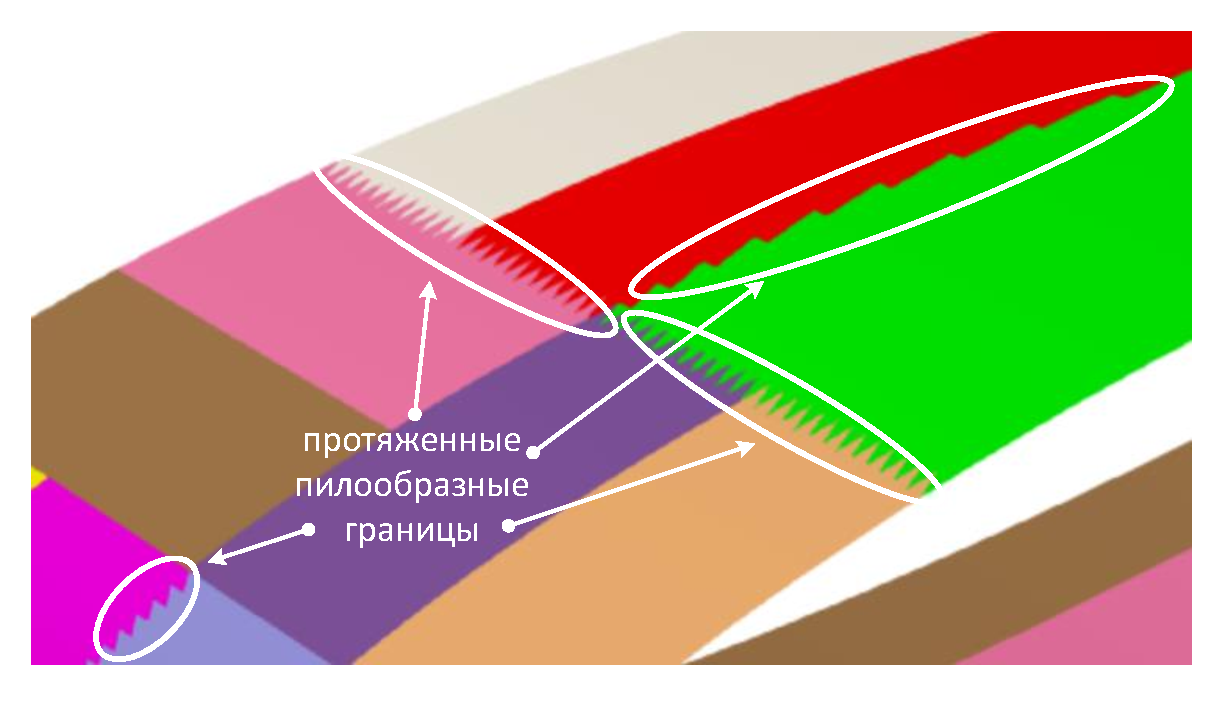
\includegraphics[width=0.6\textwidth]{./pics/text_2_smooth/bad-border.pdf}
\singlespacing
\captionstyle{center}\caption{Возникновение протяженных пилообразных границ между доменами.}
\label{fig:text_2_smooth_bad_border}
\end{figure}

Конечно такие границы необходимо отдельно обрабатывать с целью сокращения их длины.
При использовании алгоритмов декомпозиции, основанных на наращивании доменов путем обхода графа в ширину, образуются более сглаженные границы, однако из-за этого деградирует параметр качества декомпозиции $D$.
Возникновение протяженных пилообразных границ между доменами особенно характерно для неструктурированных поверхностных сеток, на которых зачастую встречаются ячейки с очень острыми углами.
Будем рассматривать алгоритм сглаживания границ между доменами, на который дополнительно накладывается требование сохранения параметра $D$.

\subsubsection{Алгоритм сглаживания границ между доменами}

Алгоритм сглаживания носит локальный характер, он применяется последовательно к каждой паре доменов и направлен на уменьшение длины границы между ними с сохранением баланса количества ячеек в этих доменах.
Граница между двумя доменами может быть представлена в виде набора простых циклов и простых цепей.
При этом простой цикл может быть обработан таким же образом, как и простая цепь, с учетом совпадения первого и последнего узла этой цепи (для такого виртуального размыкания простого цикла может быть выбран произвольный узел этого цикла).
В процессе применения алгоритма сглаживания может быть выполнено виртуальное размыкание всех простых циклов, после чего все образовавшиеся цепи рассматриваются последовательно.
Без ограничения общности можно считать, что мы работаем с одной простой цепью (полученной с помощью записи всех отдельных простых цепей подряд), представляющей границу между парами доменов.

Вначале одним линейным проходом по цепи выполняется поиск всех пригодных для оптимизации границы шаблонов, представленных на рис.~\ref{fig:text_2_smooth_smooth_border}.

\begin{figure}[ht]
\centering
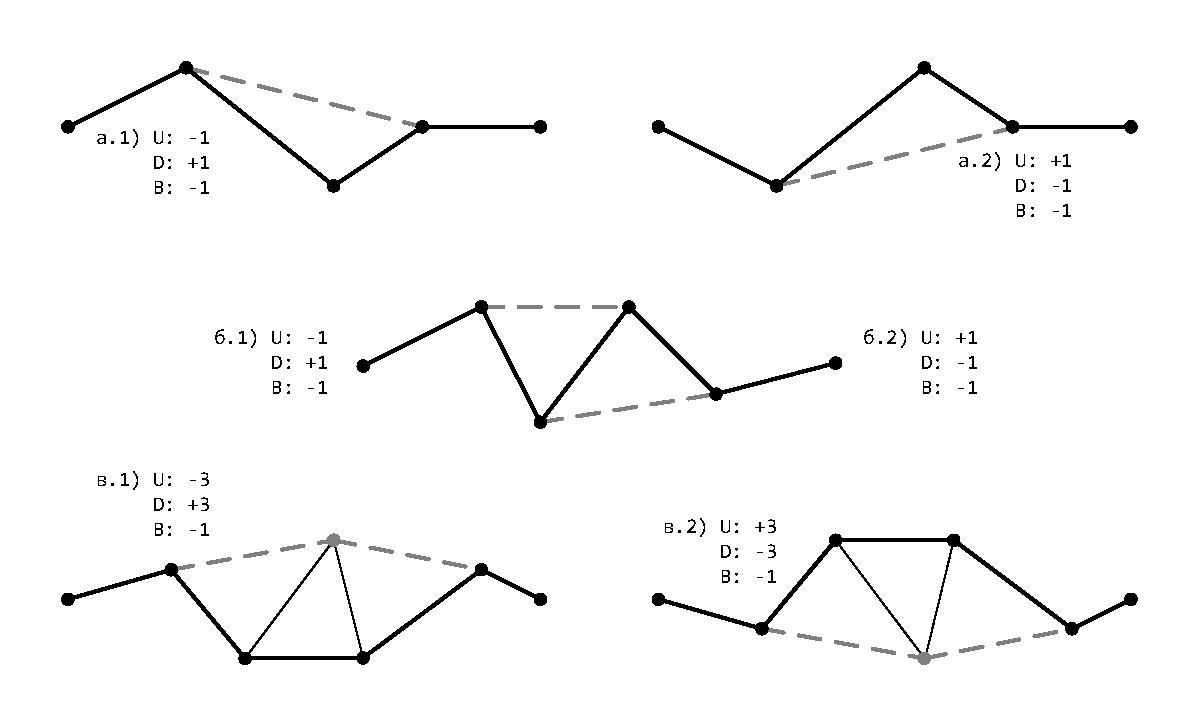
\includegraphics[width=0.8\textwidth]{./pics/text_2_smooth/smooth-border.pdf}
\singlespacing
\captionstyle{center}\caption{Шаблоны элементарных действий сглаживания границ между доменами.}
\label{fig:text_2_smooth_smooth_border}
\end{figure}

На рис.~\ref{fig:text_2_smooth_smooth_border} представлены 5 шаблонов, которые мы будем использовать для оптимизации длины границы между двумя доменами.
Рассмотрим шаблон а.1.
На нем обозначена часть границы между двумя доменами (домен сверху от ломаной обозначен буквой $U$, домен снизу от ломаной обозначен буквой $D$.
Черной сплошной линией прочерчена текущая граница между доменами.
Пунктирной линией показано возможное улучшение, которое в данном случае приведет к следующим последствиям: уменьшение количества ячеек верхнего домена на 1 ($U: -1$), увеличение количества ячеек нижнего домена на 1 ($D: + 1$), уменьшение длины границы между двумя доменами на 1 ($B: -1$).
Таким образом, шаблон а.1 направлен на втягивание одной ячейки из верхнего домена в нижний домен с сокращением длины границы на единицу.
Шаблон а.2 выполняет симметричное действие по втягиванию одной ячейки из нижнего домена в верхний домен, также сокращая при этом длину границы на единицу.
Шаблоны в.1 и в.2 выполняют аналогичные действия, однако вместо одной ячейки происходит втягивание сразу трех соседних ячеек с одновременным уменьшением длины границы между доменами на единицу. Отдельно стоит отметить шаблоны б.1 и б.2.
Они представляют собой один шаблон в рамках которого может быть осуществлено втягивание либо ячейки из нижнего домена в верхний, либо наоборот, но не одновременно (в противном случае длина границы останется неизменной).
Можно рассматривать и более сложные шаблоны, однако существенного прироста производительности они уже не дают, но приводят к усложнению алгоритма.

После того, как внутри цепи найдены все шаблоны, потенциально пригодные для оптимизации границы, выполняется разметка того, как данные шаблоны могут влиять на другие шаблоны.
С учетом того, что любой шаблон может повлиять только на своих непосредственных соседей, такое действие также выполняется с линейной сложностью относительно длины границы.

Последним шагом применения алгоритма является выбор такого множества шаблонов, которые не влияют друг на друга (то есть могут быть применены все одновременно) и не нарушают суммарного баланса ячеек (так как для нас важнейшим показателем эффективности декомпозиции расчетной сетки является равномерность распределения ячеек по доменам).
После выбора наибольшего возможного набора шаблонов они применяются, и на этом обработка цепи считается завершенной.

Рассмотрим более подробно алгоритм выбора максимального подмножества неконфликтующих шаблонов, не нарушающих общий баланс ячеек между парой доменов.
Для этого рассмотрим пример, представленный на рис.~\ref{fig:text_2_smooth_smooth}

\begin{figure}[ht]
\centering
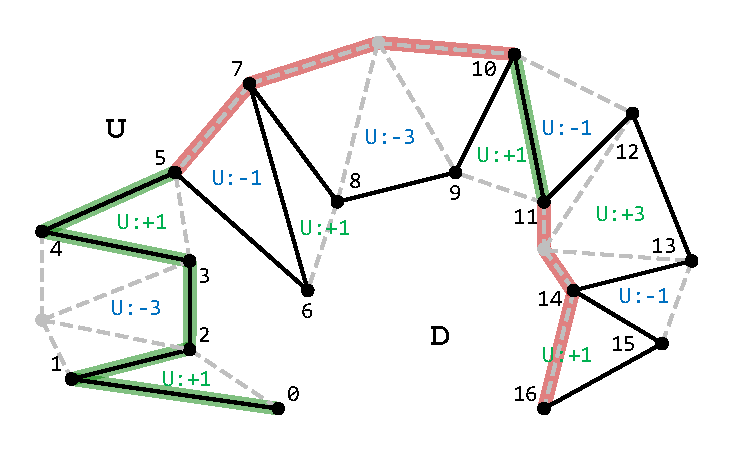
\includegraphics[width=0.8\textwidth]{./pics/text_2_smooth/smooth.pdf}
\singlespacing
\captionstyle{center}\caption{Алгоритм сглаживания границы между доменами.}
\label{fig:text_2_smooth_smooth}
\end{figure}

На рис.~\ref{fig:text_2_smooth_smooth} представлена граница между двумя доменами (они условно обозначены $U$ -- верхний и $D$ -- нижний) в виде простой цепи $0-16$.
Шаблон, который может быть применен для сглаживания границы будем обозначать $t_{a-b}$, где $a$ -- номер стартовой вершины, а $b$ -- номер конечной вершины ($b > a$).
На рис.~\ref{fig:text_2_smooth_smooth} представлены следующие шаблоны
\begin{equation}
T = \{ t_{0-2}, t_{1-4}, t_{3-5}, t_{5-7}, t_{6-8}, t_{7-10}, t_{9-11}, t_{10-12}, t_{11-14}, t_{13-15}, t_{14-16} \}
\end{equation}

Использование каждого из приведенных шаблонов уменьшает длину границы, но нарушает баланс ячеек между доменами.
Будем использовать функцию $U(t)$, которая обозначает изменение баланса ячеек по отношению к домену $U$ из-за применения шаблона $t$.
Так $U(t_{7-10}) = -3$, что означает, что при применении шаблона $t_{7-10}$ домен $U$ потеряет 3 ячейки.

\begin{definition}
Пусть даны два шаблона $t_{a-b}$ и $t_{c-d}$.
Будем говорить, что $t_{a-b} = t_{c-d}$, если $a = c$, $b = d$.
Также будем говорить, что $t_{a-b} < t_{c-d}$, если $a < c$.
\end{definition}

\begin{definition}
Два шаблона $t_{a-b} < t_{c-d}$ назовем конфликтующими (или пересекающимися по ребрам), если $c < b$, и будем обозначать $t_{a-b} \cap t_{c-d} \ne \emptyset$.
\end{definition}

На рис.~\ref{fig:text_2_smooth_smooth} каждая пара соседних шаблонов кроме $t_{3-5}$, $t_{5-7}$ является конфликтующей.
Два конфликтующих шаблона применить одновременно нельзя, так как это не приведет к уменьшению длины границы.

Ввиду того, что применение каждого отдельного шаблона уменьшает длину границы на 1, задача поиска оптимального решения может быть сформулирована в виде поиска в множестве шаблонов подмножества максимального размера, не содержащего конфликтующих шаблонов.
Поставленную задачу будем решать методом динамического программирования (схема работы алгоритма для примера с рис.~\ref{fig:text_2_smooth_smooth} представлена на рис.~\ref{fig:text_2_smooth_smooth_scheme}).
Для этого рассмотрим функцию $B(t, u, x)$, отражающую изменение длины границы при решении задачи на множестве шаблонов $\{ t' \in T : t' \ge t \}$ при условии изменения количества ячеек в домене $U$ на $u$ единиц.
Параметр $x$ является булевым и принимает значение $1$, если шаблон $t$ вошел в решение, и $0$ -- в противном случае.
Решением поставленной задачи является значение $\min(B(t_0, 0, 1), B(t_0, 0, 0))$, где $t_0$ -- первый шаблон на рассматриваемой цепи, в нашем случае это $t_{0-2}$.

\begin{figure}[!ht]
\centering
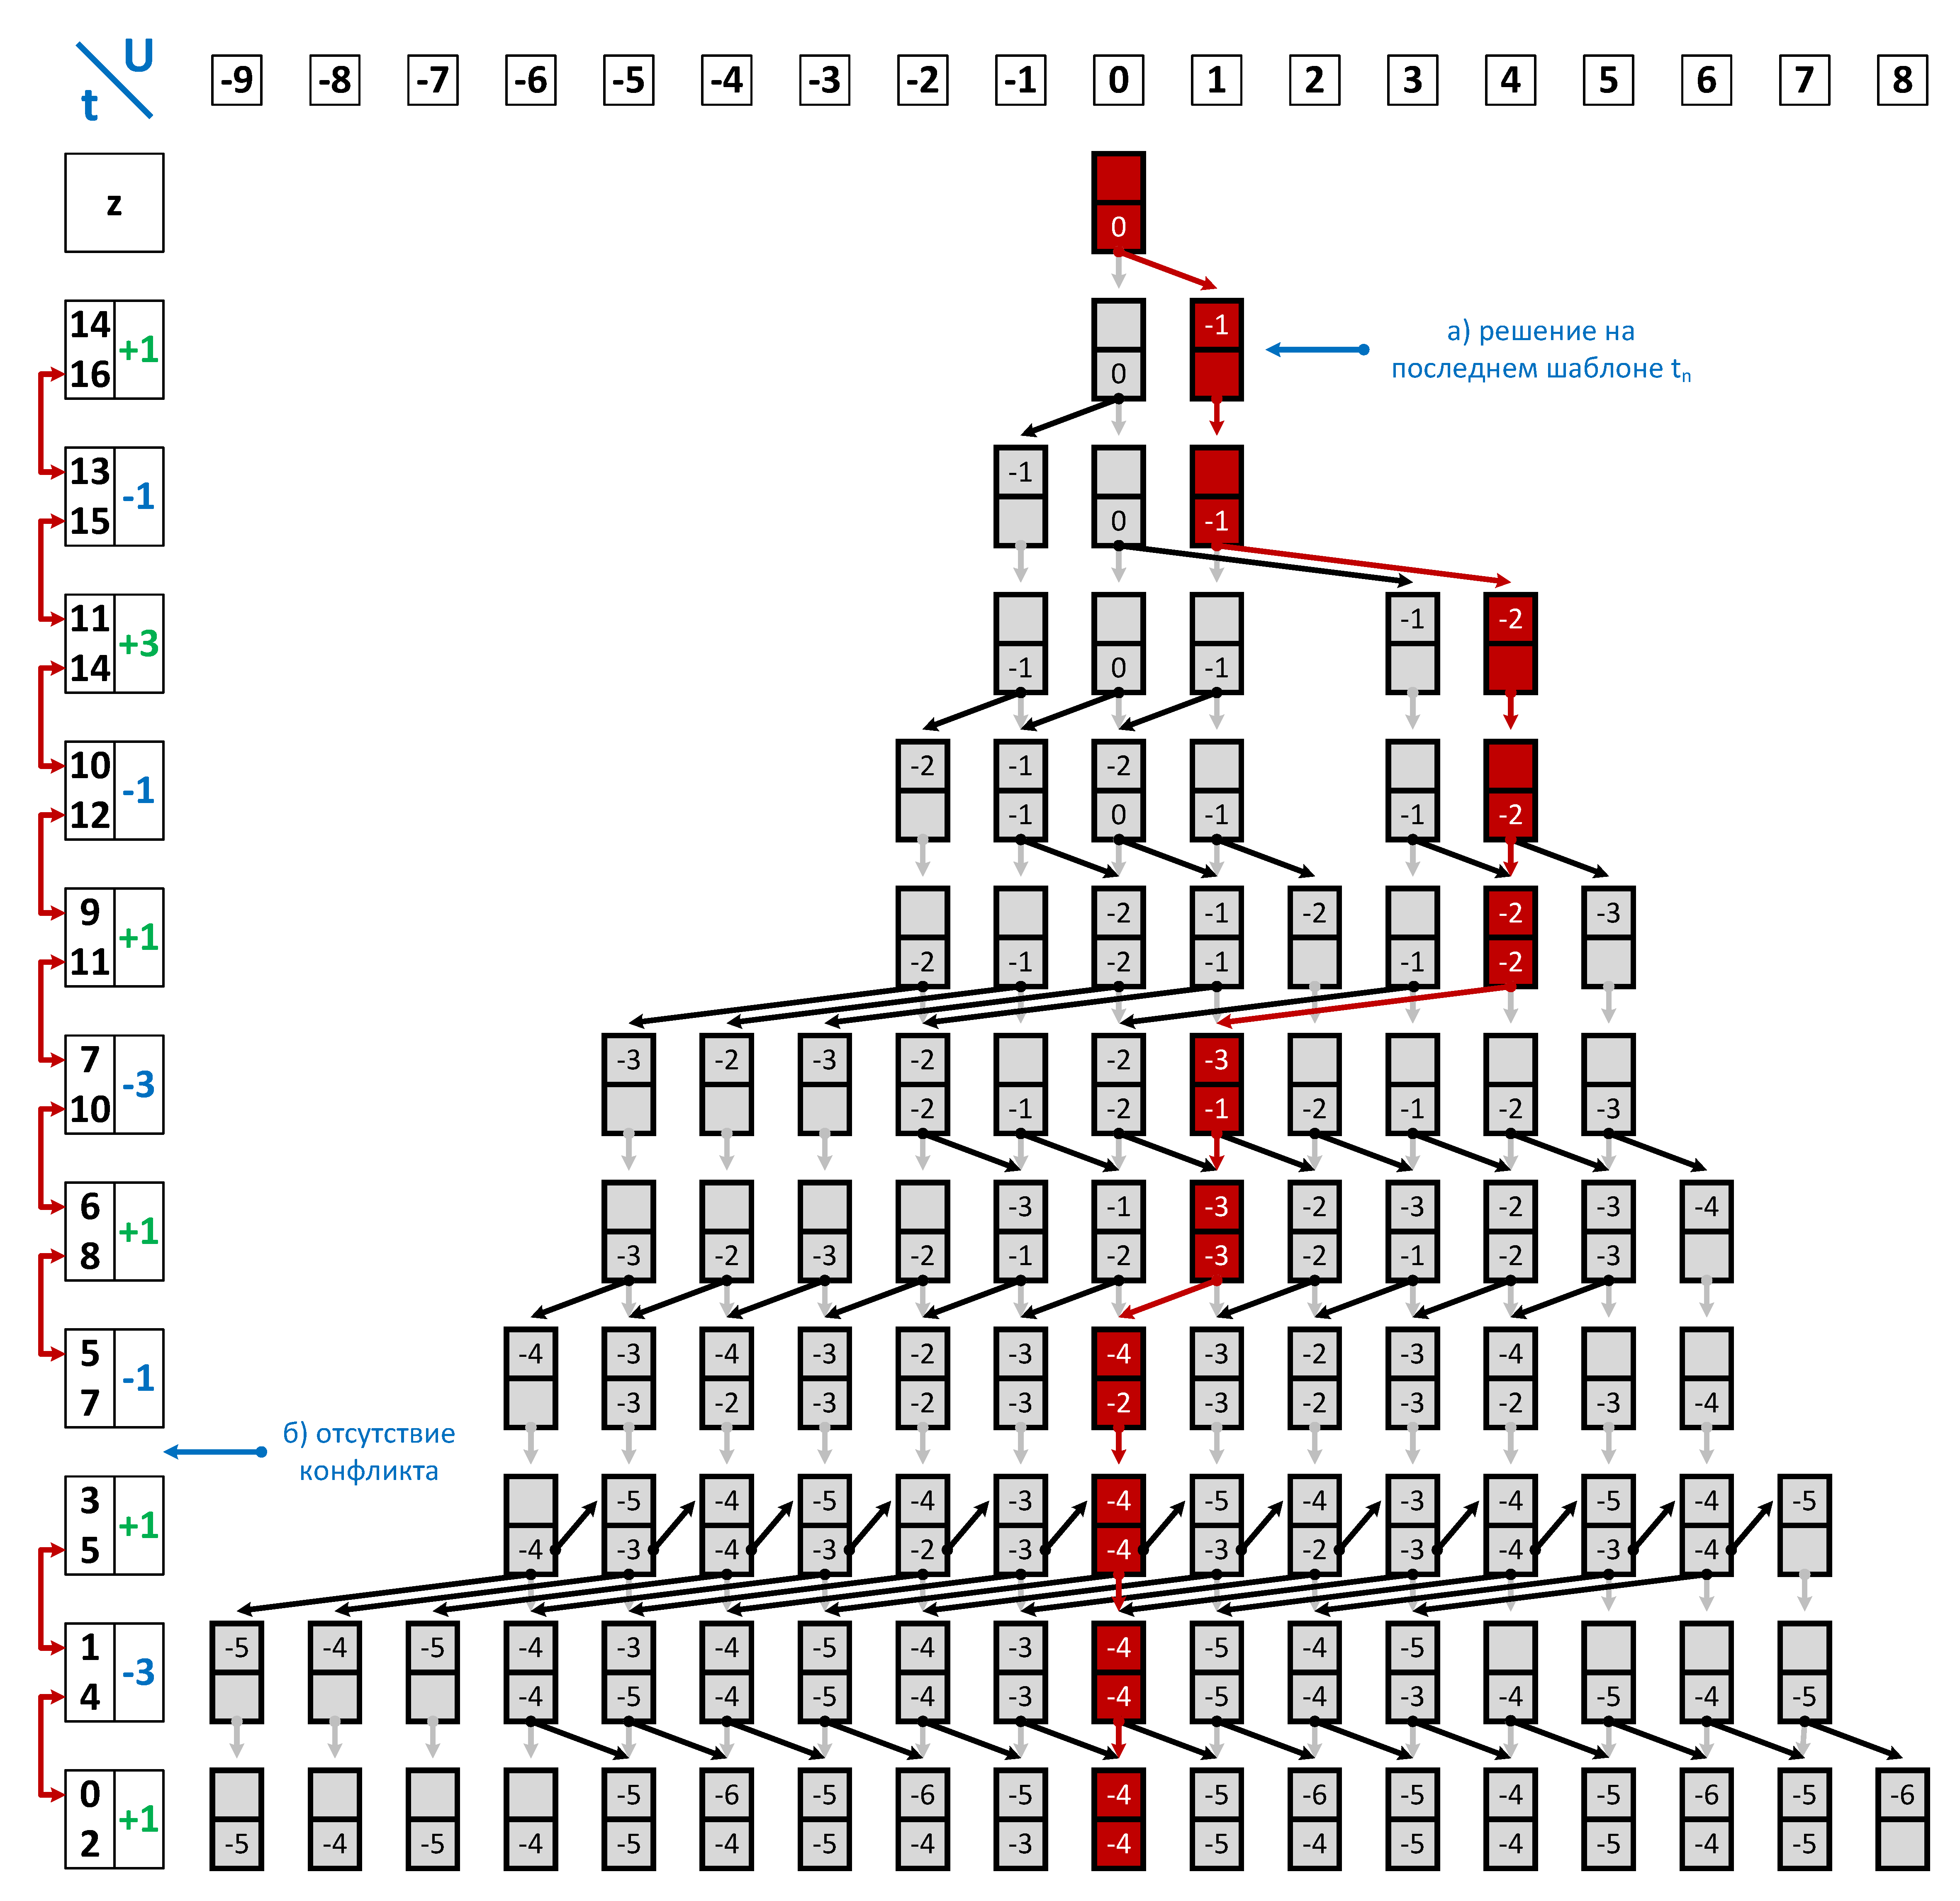
\includegraphics[width=1.0\textwidth]{./pics/text_2_smooth/smooth-scheme-cut.pdf}
\singlespacing
\captionstyle{center}\caption{Схема поиска решения задачи сглаживания границы между доменами.}
\label{fig:text_2_smooth_smooth_scheme}
\end{figure}

Решение задачи начинается с последнего шаблона $t_n$ (в нашем случае это $t_{14-16}$) (см. рис.~\ref{fig:text_2_smooth_smooth_scheme}, а).
Для него все множество используемых шаблонов состоит только из него самого, и
\begin{equation}
	\left\{
		\begin{aligned}
			& B(t_n, 0, 0) = 0 \\
			& B(t_n, U(t_n), 1) = -1
		\end{aligned}
	\right.
\end{equation}

для всех остальных значений $u$ значение функции $B(t_n, u, x)$ не определено, будем считать его равным $+\infty$.

Пусть задача решена для некоторого шаблона $t_{k + 1}$.
Рассмотрим переход к решению для $t_k$.
Изначатьно все значения $B(t_k, u, x)$ принимаются равными $+\infty$.

Во-первых, имея любое допустимое решение для шаблона $t_{k + 1}$ мы можем получить решение для шаблона $t_k$, просто проигнорировав этот шаблон, то есть для всех $u$, для которых найдено решение для шаблона $t_{k + 1}$, выполним следующую операцию (на рис.~\ref{fig:text_2_smooth_smooth_scheme} представлена серыми стрелками):
\begin{equation}
	B(t_k, u, 0) = \min \left( B(t_{k + 1}, u, 0), B(t_{k + 1}, u, 1) \right)
\end{equation}

Игнорирование шаблона $t_k$ не меняет баланс ячеек между доменами, из рис.~\ref{fig:text_2_smooth_smooth_scheme} это видно, так как все серые стрелки направлены строго вниз.

Второй момент связан с попыткой использования шаблона $t_k$.
Если $t_k \cap t_{k + 1} = \emptyset$, то есть конфликта нет (см. рис.~\ref{fig:text_2_smooth_smooth_scheme}, б), то шаблон $t_k$ можно использовать вне зависимости от того, был ли использован шаблон $t_{k + 1}$.
То есть для всех $u$, для которых было найдено решение для шаблона $t_{k + 1}$ выполним следующее действие:
\begin{equation}
	B(t_k, u + U(t_k), 1) = B(t_k, u, 0) - 1
\end{equation}

И наконец в случае конфликтующих $t_k$ и $t_{k + 1}$ мы можем использовать шаблон $t_k$ только в том случае, если не был использован шаблон $t_{k + 1}$, то есть для всех $u$ для которых $B(t_{k + 1}, u, 0) \ne +\infty$ нужно выполнить операцию
\begin{equation}
	B(t_k, u + U(t_k), 1) = B(t_{k + 1}, u, 0) - 1
\end{equation}

В результате работы алгоритма получим все наилучшие варианты использования шаблонов для заданного изменения баланса ячеек между доменами $U$ и $D$, в частности для нулевого изменения баланса.
На рис.~\ref{fig:text_2_smooth_smooth_scheme} красным цветом выделен путь для достижения наилучшего сокращения пути при сохранении баланса ячеек между доменами.
В нашем случае одним (но не единственным) из оптимальных решений является использование шаблонов $t_{14-16}$, $t_{11-14}$, $t_{7-10}$, $t_{5-7}$, что сокращает границу между доменами на 4, это решение отражено на рис.~\ref{fig:text_2_smooth_smooth}.

В результате работы алгоритма рассчитываются оптимальные решения для всех значений $u$ из диапазона
\begin{equation}
	[U_{min}, U_{max}] = \left[ \frac{1}{2} \sum_{t \in T}{(U(t) - |U(t)|)}, \frac{1}{2} \sum_{t \in T}{(U(t) + |U(t)|)} \right]
\end{equation}

и его сложность равна $O \left( |T| \cdot (U_{max} - U_{min} + 1) \right)$.

\begin{figure}[ht]
\centering
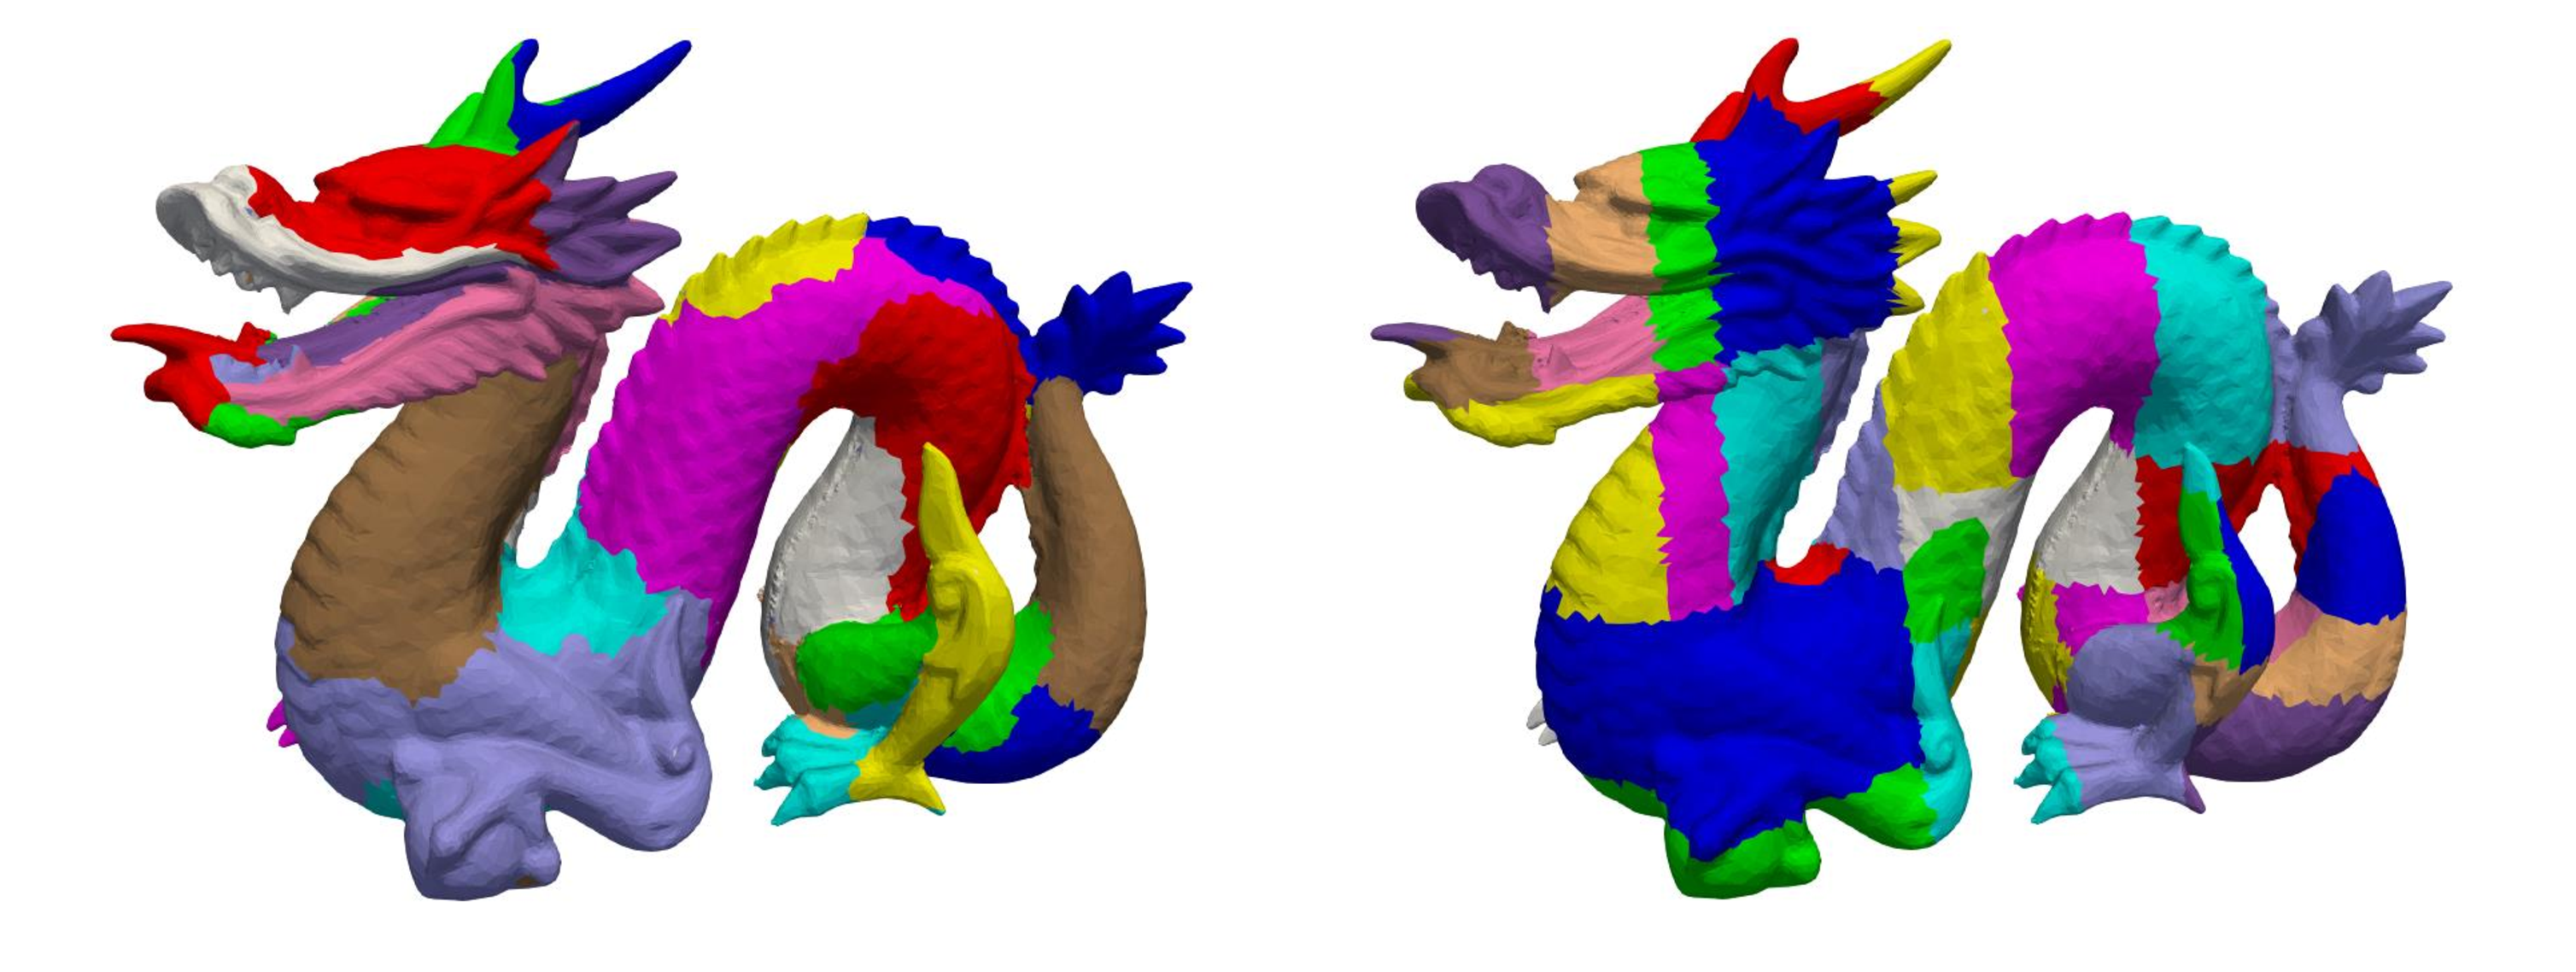
\includegraphics[width=1.0\textwidth]{./pics/text_2_smooth/decomp.pdf}
\singlespacing
\captionstyle{center}\caption{Визуализация декомпозиции тестовой расчетной сетки dragon на 32 домена с помощью алгоритма Фархата (слева) и иерархического алгоритма (справа).}
\label{fig:text_2_smooth_decomp}
\end{figure}

\begin{figure}[ht]
\centering
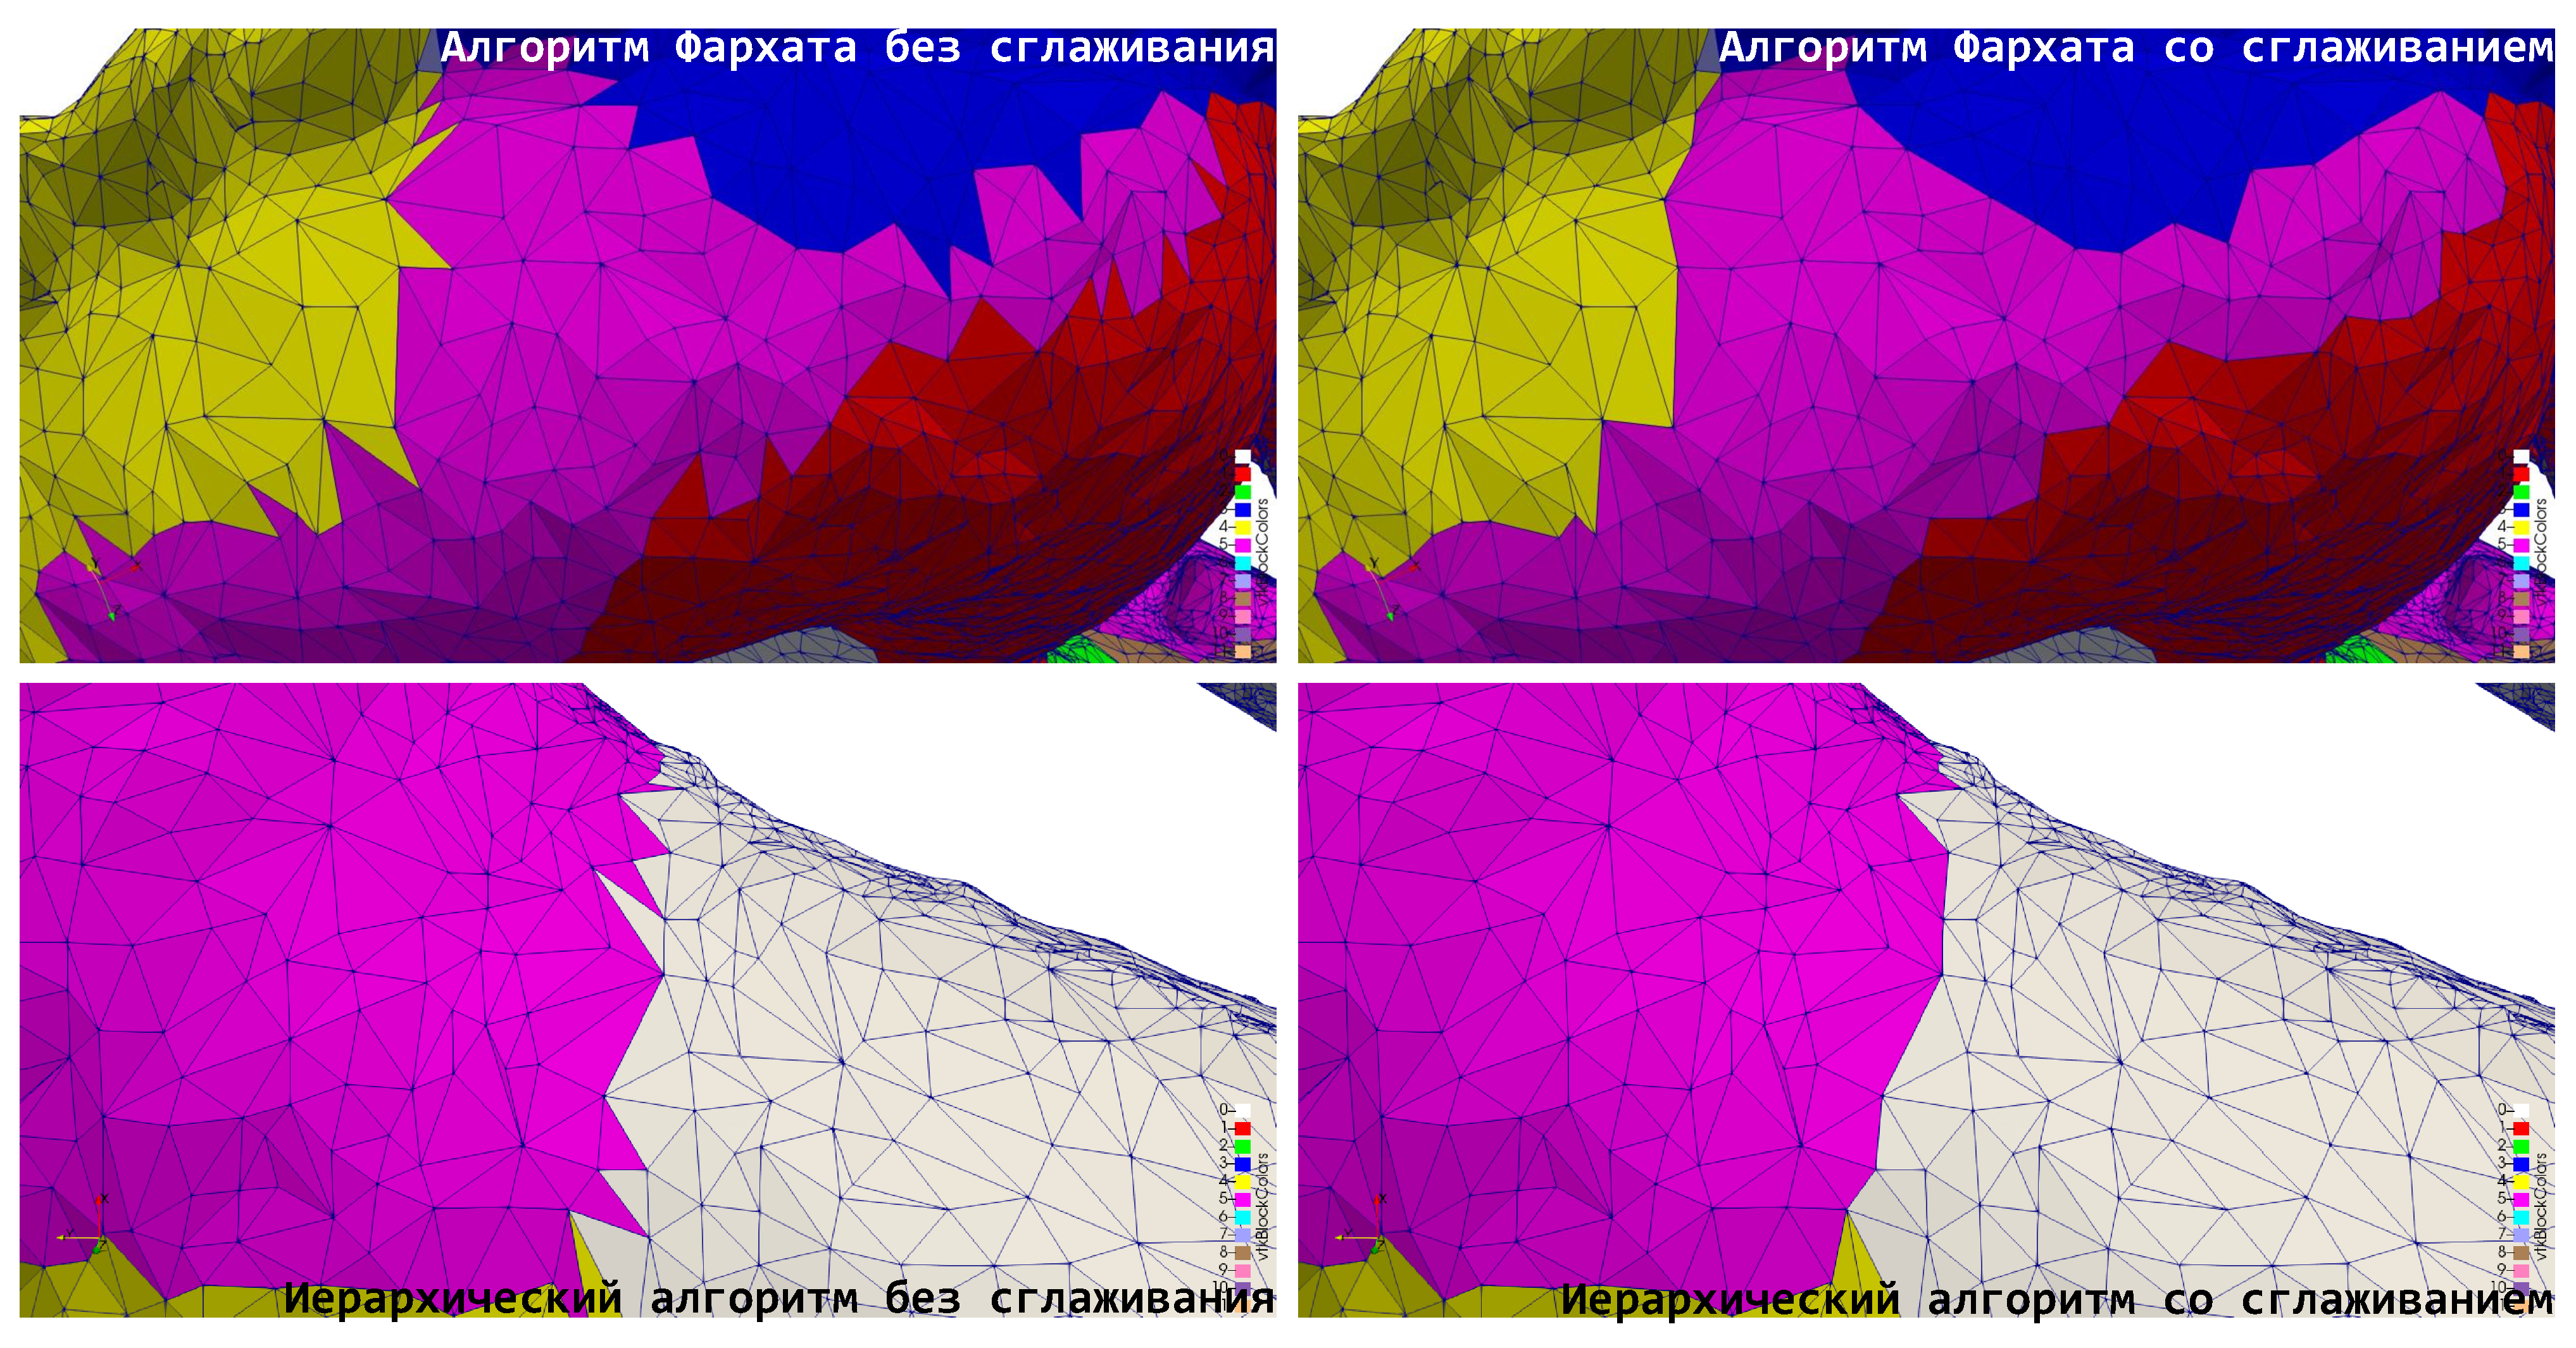
\includegraphics[width=0.8\textwidth]{./pics/text_2_smooth/decomp2.pdf}
\singlespacing
\captionstyle{center}\caption{Визуализация применения сглаживания границ между доменами после работы алгоритма Фархата (сверху) и иерархического алгоритма (снизу).}
\label{fig:text_2_smooth_decomp2}
\end{figure}

На рис.~\ref{fig:text_2_smooth_decomp} представлена визуализация декомпозиции тестовой расчетной сетки dragon с помощью алгоритма Фархата и иерархического алгоритма бинарной декомпозиции.
В обоих случаях декомпозиция выполнятся на 32 домена.
При этом на рис.~\ref{fig:text_2_smooth_decomp2} представлены результаты работы с уже примененным сглаживанием границ между доменами.

На рис.~\ref{fig:text_2_smooth_decomp2} крупным планом продемонстрированы отдельные части тестовой расчетной сетки dragon с отображением ребер ячеек.
На этом рисунке виден эффект от применения алгоритма сглаживания границ меду доменами, прежде всего от заключается в устранении одиноких ячеек, которые вторгаются в соседний домен одной своей вершиной.
После применения алгоритма границы между доменами визуально выглядят более гладко, их длина уменьшается.

\subsubsection{Результаты экспериментов}

Для тестирования эффективности алгоритма сглаживания границ между доменами использовались тестовые неструктурированные поверхностные сетки bunny, dragon, lucy, к которым были применены алгоритмы декомпозиции с показателем $D = 0$ и сравнены показатели качества декомпозиции до и после сглаживания границ.
Результаты проведения экспериментов представлены на рис.~\ref{fig:text_2_smooth_graphics}.

\begin{figure}[H]
\centering
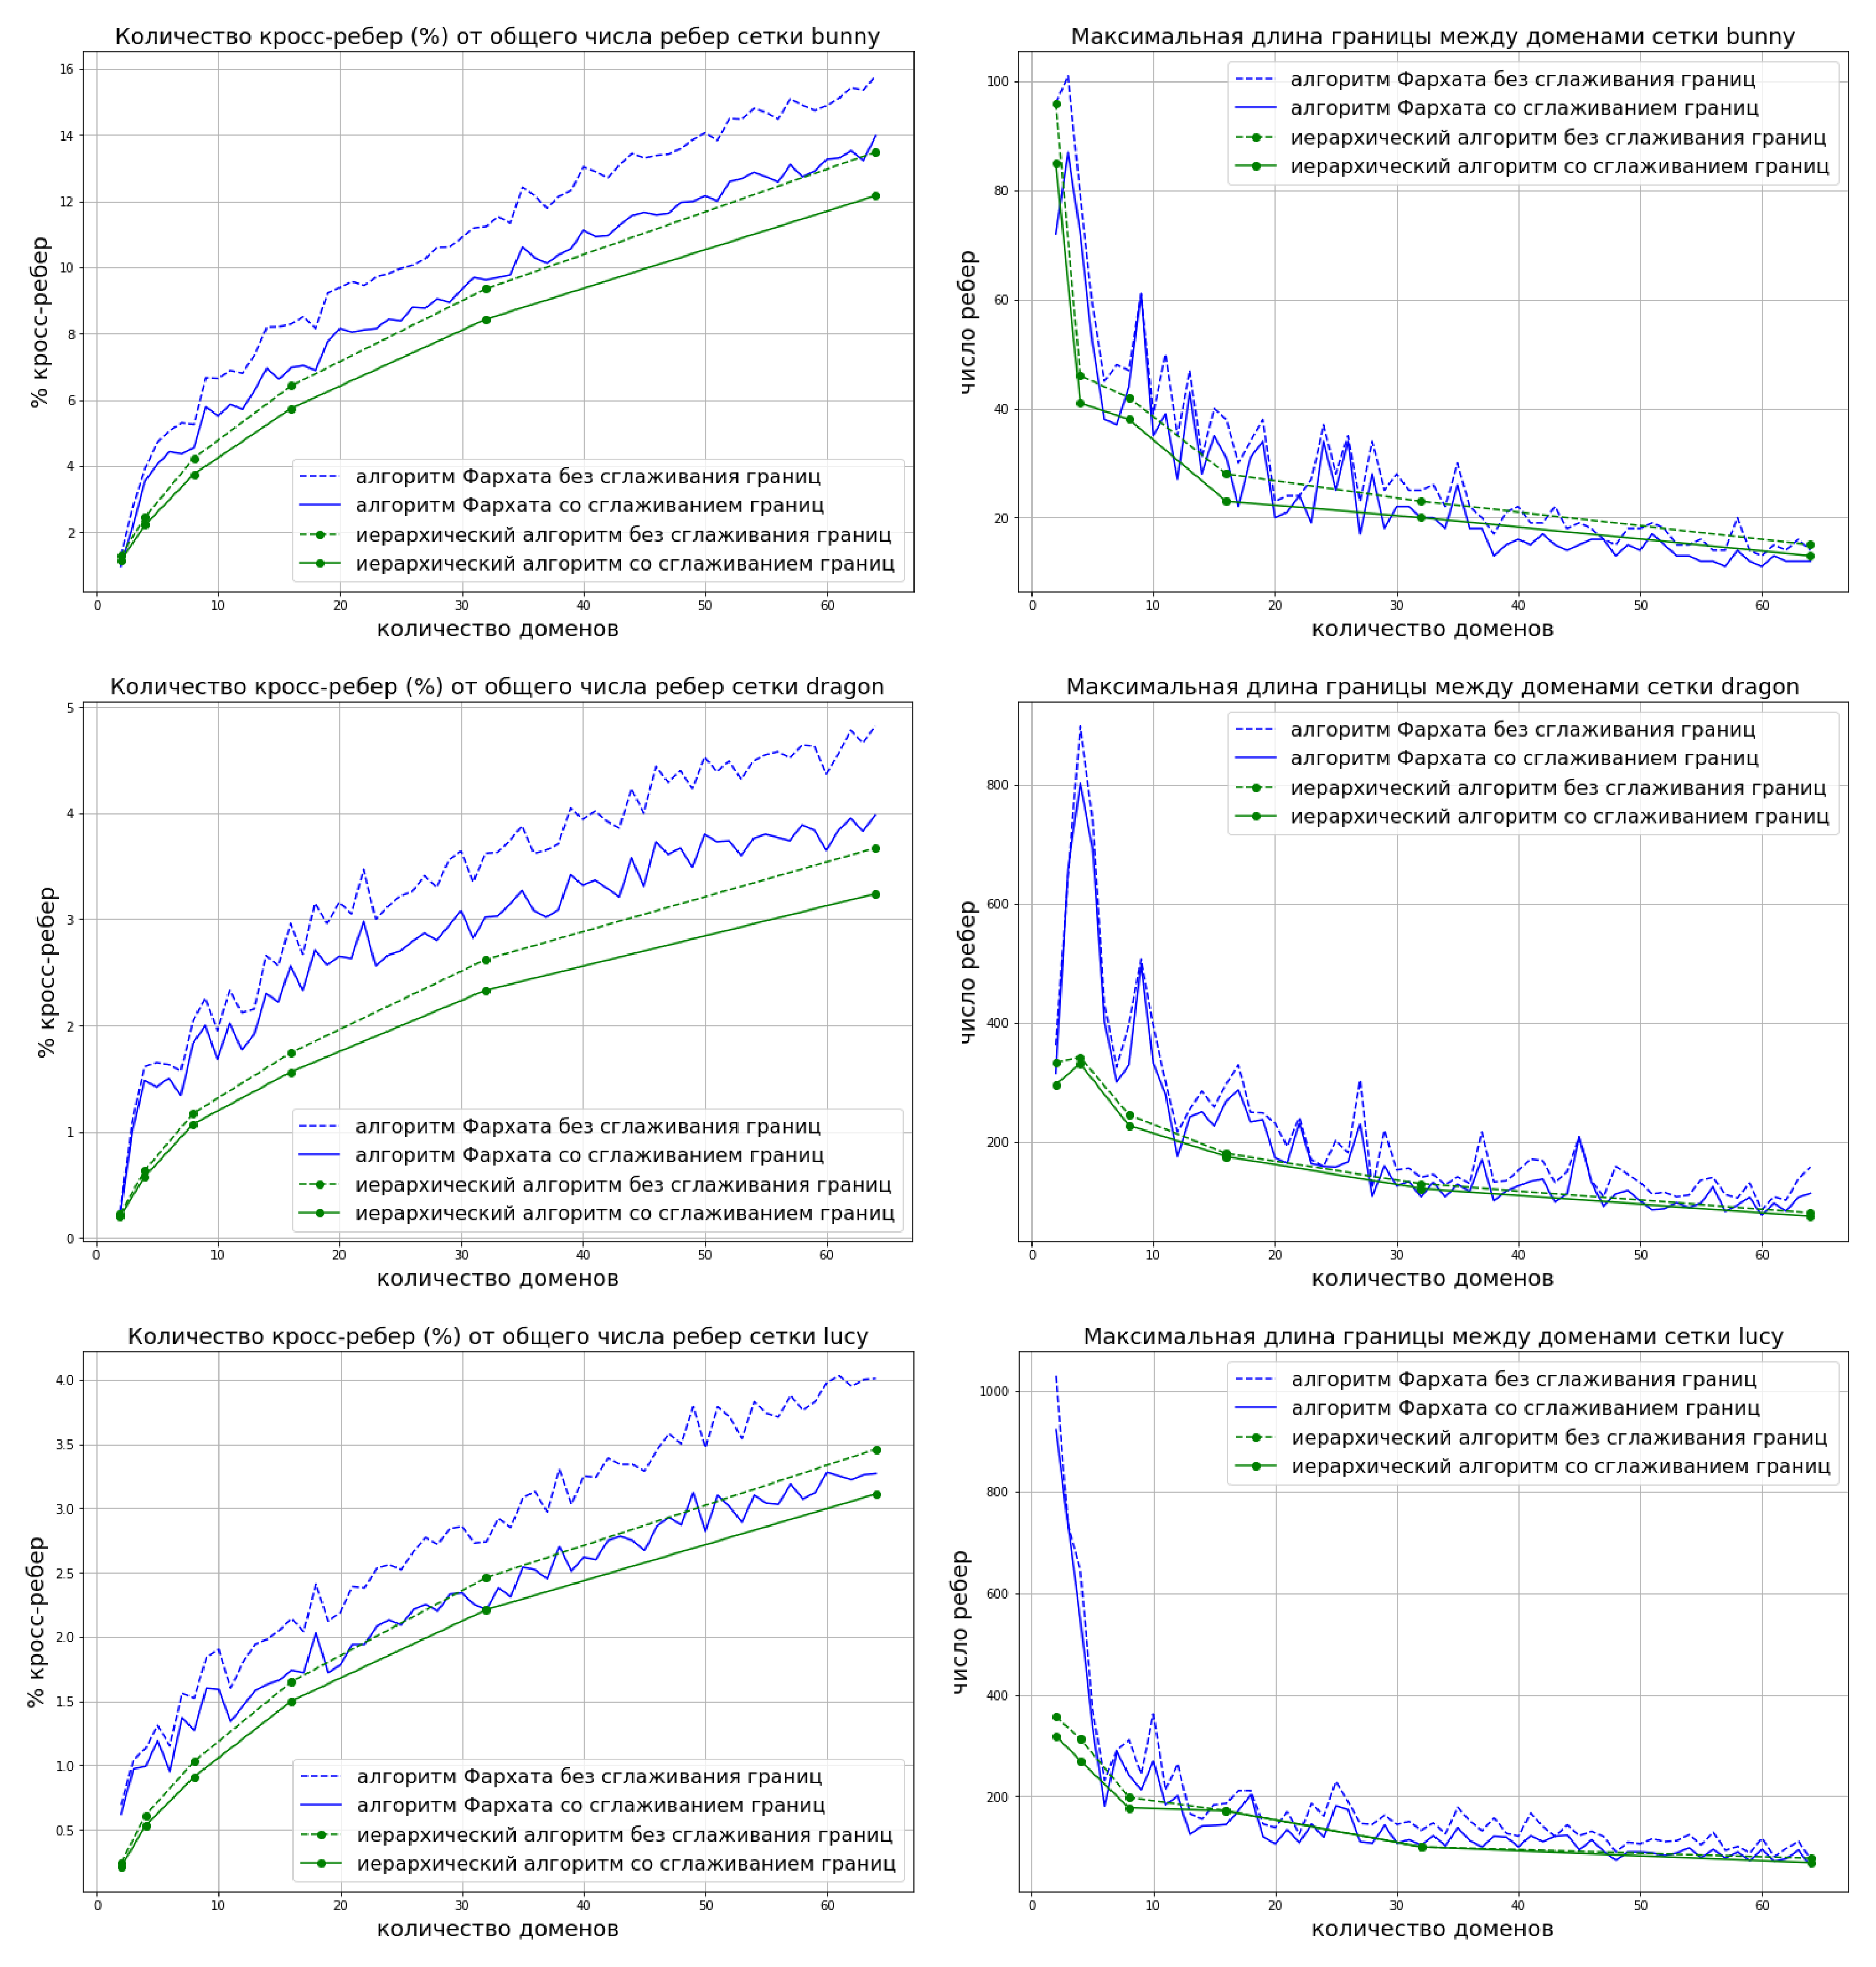
\includegraphics[width=1.0\textwidth]{./pics/text_2_smooth/graphics.pdf}
\singlespacing
\captionstyle{center}\caption{Графики доли кросс-ребер от общего числа ребер сетки (показатель $I^{\%}$) и максимальной длины границы между доменами (показатель $L$) при декомпозиции тестовых сеток bunny, dragon и lucy на количество доменов от 2 до 64.}
\label{fig:text_2_smooth_graphics}
\end{figure}

Неструктурированные поверхностные расчетные сетки bunny (количество ячеек $5 \cdot 10^3$), dragon (количество ячеек $10^5$), lucy (количество ячеек $10^5$) были взяты из открытых источников.
Из приведенных на рис.~\ref{fig:text_2_smooth_graphics} данных видно, что в целом проиллюстрированные показатели эффективности декомпозиции расчетных сеток (процентная доля ребер сетки, являющихся граничными ребрами между доменами, и максимальная длина границы между доменами) лучше для иерархического пространственного алгоритма декомпозиции.
Применение же алгоритма сглаживания границ приводит к сокращению как общего количества граничных ребер (кросс-ребер), так и длины максимальной границы примерно на 10\%.
Этот эффект приводит к снижению времени межпроцессных обменов для задач, выполняющих расчеты на поверхностных расчетных сетках.
